% ===================================================================
\section{Donor Selection}\label{sec:donoraudit}
% ===================================================================
Donor selection is the identification step of the whole design, because the synthetic can isolate the oil-specific premium only if the pool reproduces Brent through the factors it
shares with many assets while carrying none of Brent's own oil-supply exposure. In this
section we build that pool by first identifying the common factors that drive Brent and the
non-oil series that proxy each. Next, we curate the candidate set against a carefully constructed set of selection criteria. Finally, we confirm with donor-level tests that the qualitative reasoning behind it
holds. 

\subsection{Donor categories and their non-oil proxies}
Brent's log price splits into a part driven by global macro-financial factors common to many
assets and an oil-specific part (Section~\ref{sec:theory}). A donor is useful when it shares
Brent's loading on the common factors but carries no loading on the oil-specific component,
because only then does it track Brent before the event and decouple when the oil shock
fires. Five factors drive Brent in normal times, and each has a set of non-oil proxies that
define the donor categories (Table~\ref{tab:factors}).

\begin{table}[h]
\centering
\caption{Common factors driving Brent and their non-oil donor proxies.}
\label{tab:factors}
\begin{threeparttable}
\small
\begin{tabular}{@{}p{3.1cm}p{5.3cm}p{5.3cm}@{}}
\toprule
Common factor & Economic channel to Brent & Non-oil donor proxies \\
\midrule
Global growth / industrial cycle & Oil demand is procyclical, moving with global industrial production and trade & Copper, Iron Ore, broad equities, commodity-exporter FX \\
US dollar & Oil is dollar-priced, so a stronger dollar lowers its dollar price & the FX block, Gold, DXY (excluded for Russia) \\
Real rates / monetary policy & Discount rate and carry on a storable commodity, the global liquidity cycle & TLT, US 10-year yield (Mild), Gold \\
Global risk appetite & Oil is a risk asset and sells off alongside equities and credit when risk turns & VIX (inverse), HYG, S\&P~500, safe-haven JPY and CHF \\
China demand & China is the marginal buyer of crude and of many commodities & Iron Ore, Copper, Soybeans, CNY, AUD \\
\bottomrule
\end{tabular}
\begin{tablenotes}[flushleft]
\footnotesize
\item \textit{Notes.} The pool spans all five factors so the synthetic can reproduce Brent under any mix of drivers, not just one. A series in parentheses is excluded for the event noted. 
\end{tablenotes}
\end{threeparttable}
\end{table}

Industrial and precious metals carry the global growth
and real-rate channels through copper, iron ore, gold and silver, whose supply has nothing
to do with Gulf or Russian crude. Agriculturals move with global demand and the dollar
through the financialised commodity complex, with production concentrated outside the oil
chokepoints. Broad equities price global growth and the equity risk premium, with energy
only a small index weight. The currency block carries the dollar factor that every non-USD
pair shares with dollar-priced oil, together with terms-of-trade and risk channels for
commodity exporters and safe havens. Long Treasuries and high-yield credit carry the
discount-rate and risk-premium factors, and the VIX carries risk appetite in its purest
inverse form. None of the retained series is itself set by oil.

\subsection{Selection criteria}
\begin{figure}[h]
\centering
\caption{Donor selection funnel.}
\label{fig:waterfall}
% Donor selection funnel (Section Donor Selection).
% Requires in the preamble: \usepackage{tikz}  \usepackage{xcolor}
\definecolor{funfill}{HTML}{6E8CAE}
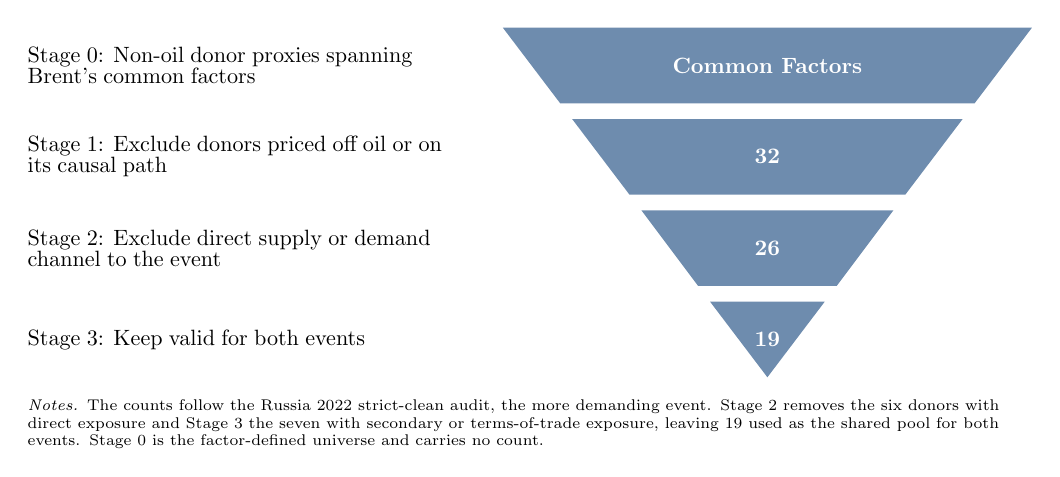
\begin{tikzpicture}[scale=0.8,transform shape,font=\footnotesize,
   bar/.style={anchor=west,align=left,text width=7.0cm,inner sep=0pt}]
  \def\cx{12}
  % inverted funnel, taper slope ~0.76; apex (cx,0.5), bands 1.2 tall with 0.25 gaps

  % ---- stage 0 : global categories (label only, the donor universe) ----
  \fill[funfill] (\cx-4.2,6.05) -- (\cx+4.2,6.05) -- (\cx+3.29,4.85) -- (\cx-3.29,4.85) -- cycle;
  \node[white,font=\normalsize\bfseries] at (\cx,5.45) {Common Factors};
  \node[bar] at (0.25,5.45) {{\normalsize Stage 0: Non-oil donor proxies spanning Brent's common factors}};

  % ---- stage 1 : 32 ----
  \fill[funfill] (\cx-3.1,4.6) -- (\cx+3.1,4.6) -- (\cx+2.19,3.4) -- (\cx-2.19,3.4) -- cycle;
  \node[white,font=\normalsize\bfseries] at (\cx,4.0) {32};
  \node[bar] at (0.25,4.0) {{\normalsize Stage 1: Exclude donors priced off oil or on its causal path}};

  % ---- stage 2 : 26 ----
  \fill[funfill] (\cx-2.0,3.15) -- (\cx+2.0,3.15) -- (\cx+1.1,1.95) -- (\cx-1.1,1.95) -- cycle;
  \node[white,font=\normalsize\bfseries] at (\cx,2.55) {26};
  \node[bar] at (0.25,2.55) {{\normalsize Stage 2: Exclude direct supply or demand channel to the event}};

  % ---- stage 3 : 19 (apex) ----
  \fill[funfill] (\cx-0.91,1.7) -- (\cx+0.91,1.7) -- (\cx,0.5) -- cycle;
  \node[white,font=\normalsize\bfseries] at (\cx,1.1) {19};
  \node[bar] at (0.25,1.1) {{\normalsize Stage 3: Keep valid for both events}};

  % ---- note ----
  \node[anchor=north west,align=left,text width=15.5cm,inner sep=0pt,font=\scriptsize]
     at (0.25,0.15) {\textit{Notes.} The counts follow the Russia 2022 strict-clean audit,
     the more demanding event. Stage 2 removes the six donors with direct exposure and Stage 3
     the seven with secondary or terms-of-trade exposure, leaving 19 used as the shared pool
     for both events. Stage 0 is the factor-defined universe and carries no count.};
\end{tikzpicture}

\end{figure}
The criterion that binds donor selection is that a donor stay off the path of the disruption
we are attributing. Direct supply or demand exposure to the focal event would violate SUTVA
and contaminate the very premium we are trying to measure, so we read this criterion strictly
in the three stages of the funnel in Figure~\ref{fig:waterfall}.

Stage 1 removes whole families by construction. The energy complex (WTI, Henry Hub
gas, refined products, crude inventories) is priced off the very oil shock we are measuring
and would pull the estimated premium toward zero. Petrocurrencies carry that same oil signal
in currency form, unstable currencies add domestic-crisis noise rather than shared-factor
signal, energy-heavy equity indices carry direct sector exposure, and a few series are
dropped as redundant with a cleaner proxy. None of these reaches the per-event step, and
Appendix~\ref{app:donoraudit} records each with its reason. What survives is the set of 32
candidates.

Stage 2 drops the candidates with a direct supply or demand channel to the focal
event. For Russia 2022 that is six series, the wheat and corn that Russia and Ukraine
dominate in world exports, palladium on Russia's share of supply, the euro and the dollar
basket through the European energy crisis, and Bitcoin on the sanctions-evasion narrative of
early 2022. For Hormuz 2026 nothing is physically routed through the Strait, so none is
dropped here. This leaves 26.

Stage 3keeps only the series clean for both events at once, so the same basket is a
valid counterfactual in each. The more exposed event is Russia, so this removes the seven
further series that reach Brent through a secondary or terms-of-trade channel over 2022,
namely copper, iron ore, soybeans, EM equities, sterling, the US 10-year yield, and cotton.
Because the Russia-clean set sits inside the Hormuz-clean set, the survivors stay clean for
Hormuz as well. The result is the shared 19-donor pool of Table~\ref{tab:donors}.

\begin{table}[h]
\centering
\caption{The retained shared 19-donor pool, by factor category.}
\label{tab:donors}
\begin{threeparttable}
\small
\begin{tabular}{@{}lp{10.5cm}@{}}
\toprule
Category & Donors (shared pool) \\
\midrule
Metals (3) & Silver, Platinum, Gold \\
Agriculturals (3) & Coffee, Sugar, Live Cattle \\
Equities (2) & S\&P 500, Nikkei 225 \\
Foreign exchange (8) & AUD, JPY, CHF, CNY, INR, KRW, ZAR, MXN \\
Rates \& credit (2) & TLT (long Treasuries), HYG (high-yield credit) \\
Volatility (1) & VIX (implied S\&P 500 volatility) \\
\bottomrule
\end{tabular}
\end{threeparttable}
\end{table}

\subsection{Empirical confirmation}
The donor-level battery of Section~\ref{sec:methods} confirms the audit. For Hormuz 2026, 31
of the 32 candidates agree at the cutoff, and only Cotton differs, its exclusion being an
economic causal-channel call that the contemporaneous tests are not expected to reproduce for
an indirect, lagged channel. For Russia 2022 the tests add a single flag on CNY, attributable
to the concurrent China zero-COVID dynamics rather than to the war. The only within-pre-window
relationship break the Bai--Perron procedure dates among retained donors is a single break in
the VIX on 2022-01-07, seven weeks before the cutoff (Appendix~\ref{app:breaks}), which we
read as informative rather than exclusionary since it does not recur on the analysis window
alone and dropping the VIX moves the estimate by less than one point.
